\documentclass[11pt,a4paper]{article}

\input{setup/project}
\input{setup/preamble}
\input{setup/weekly}

% The methods sections are input from ../methodology; their figures use paths from the thesis root.


\renewcommand{\reportdate}{4 November 2026}

\begin{document}

\weeklytitle{10}

\section{Week 10: 2--6 November 2026}

\sectionprogress

\begin{itemize}
  \item \textbf{I am close to locking down how to build the risk model} My top model is a
    segment-level cloglog GLMM over the 9 segments with a person random intercept, and its
    segment risks pooled into one person risk. I will keep a person-level model of any plaque as a benchmark 
  \item \textbf{A new method: Functional Principal Component Analysis (FPCA).} The mean turning angle per segment still loses information about where the bends lie even though not as much if it was computed on the full artery or at person level.
    \begin{itemize}
      \item \textbf{Profiles.} The turning profile of each segment is interpolated onto 50 positions
        along the normalised segment length, giving one matrix of people $\times$ positions.
      \item \textbf{Shapes.} The average profile is subtracted, and the singular value decomposition (SVD) gives the shapes along
        which people differ most, with one score per person and shape. 
        \item \textbf{Mean turning angle turns out to be a good summary.} On the Herlev--{\O}sterbro
        Medis profiles, the first shape has the same sign along the whole segment and is basically a striaght line, so it represents the mean turning angle. The mean turning is therefore the best single summary of the profile, even though we have no idea if mean turning correlates with plaque. Some litterature says yes, some says no. 
      \item \textbf{Where will the analysis be conducted?} Only the pLAD and mLAD have enough events for several curvature terms
        (Riley maximum 10 and 8, against at most 5 elsewhere), so the analysis is done in these two
        segments only, and it is descriptive.
      \item \textbf{Number of shapes.} Fixed before the outcome is used. 
  \item \textbf{I wrote some of the methods sections} on the in-house tracer, the Medis reference, the
    cohort and outcome, and the arteries and segments.
\end{itemize}

% Week 10: curvature shapes (FPCA) in the pLAD and mLAD, explained on made-up data. Input from week10.tex.
% Figures: fpca_steps_figures.py. Text left, figure right (minipages, so no extra package is needed).
\newcommand{\fpcarow}[2]{\par\noindent
  \begin{minipage}[t]{0.54\textwidth}\vspace{0pt}#1\end{minipage}\hfill
  \begin{minipage}[t]{0.42\textwidth}\vspace{0pt}#2\end{minipage}\par\medskip}
\newcommand{\fpcafig}[2]{\centering\includegraphics[width=\linewidth]{week_figure/fpca_steps/fake/#1}\\[-0.1em]
  {\footnotesize #2}}

\subsection*{Curvature shapes in the proximal and mid LAD (FPCA)}
In the main model, curvature is the mean turning of each segment. The mean does not say where the
vessel bends: one sharp bend and a gentle turn along the whole segment can give the same mean.
Functional principal component analysis (FPCA) finds the few main shapes in which people's turning
differs along a segment, and gives each person a score for how much of each shape they have. These
scores then replace the mean in the risk model, to see whether where the vessel bends matters, not
only how much. This is only done in the pLAD and mLAD, the only segments where enough people developed
plaque to estimate several curvature terms, and it is descriptive. The figures use made-up people.

\fpcarow{%
\textbf{Turning angle.} At each point of the centerline, one point is placed 5\,mm before it and one
5\,mm after it, in a straight line. The turning angle is the angle between the line coming in and the
line going out: how much the vessel changes direction at that point. Dividing it by the 5\,mm gives the
turning in rad/mm. Bends shorter than about 5\,mm are not seen, and the first and last 5\,mm of a
vessel get no value. It is computed along the whole
artery and then cut at the segment boundaries, so a bend across a boundary is still measured.
}{%
\centering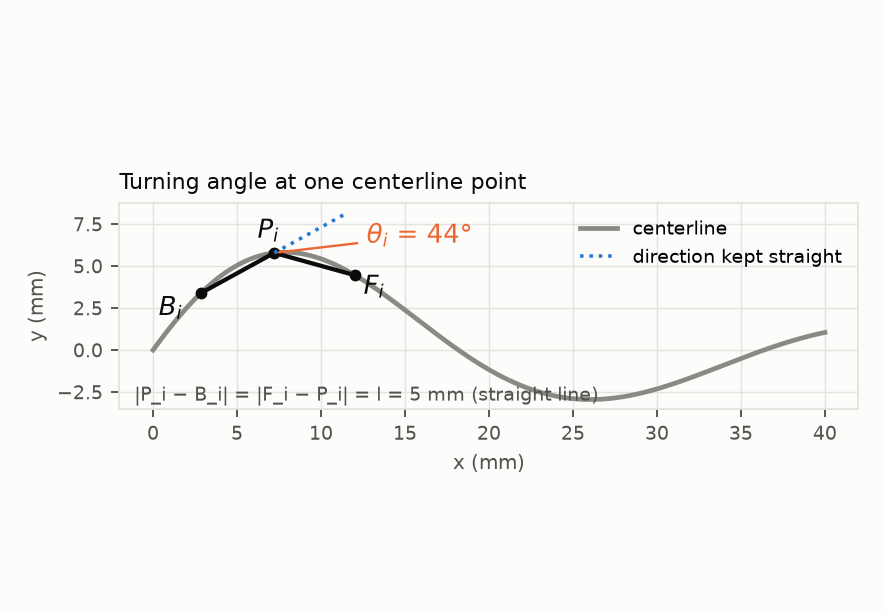
\includegraphics[width=\linewidth]{week_figure/fpca/f1_turning_geometry.png}\\[-0.1em]
{\footnotesize The turning angle $\theta_i$ at one point of a made-up centerline.}
}

\fpcarow{%
\textbf{The same 50 places for everyone.} The turning has one value per centerline point, and
segments differ in length and in how many points they have (top). To compare people place by place,
each segment is stretched or squeezed to run from 0 (start) to 1 (end), and the turning is read at the
same 50 places (bottom). Place 25 is then halfway along the segment for everyone, whether the segment
is 30 or 50\,mm long. The shapes therefore describe
where along the segment the vessel turns, not how long it is.
}{%
\centering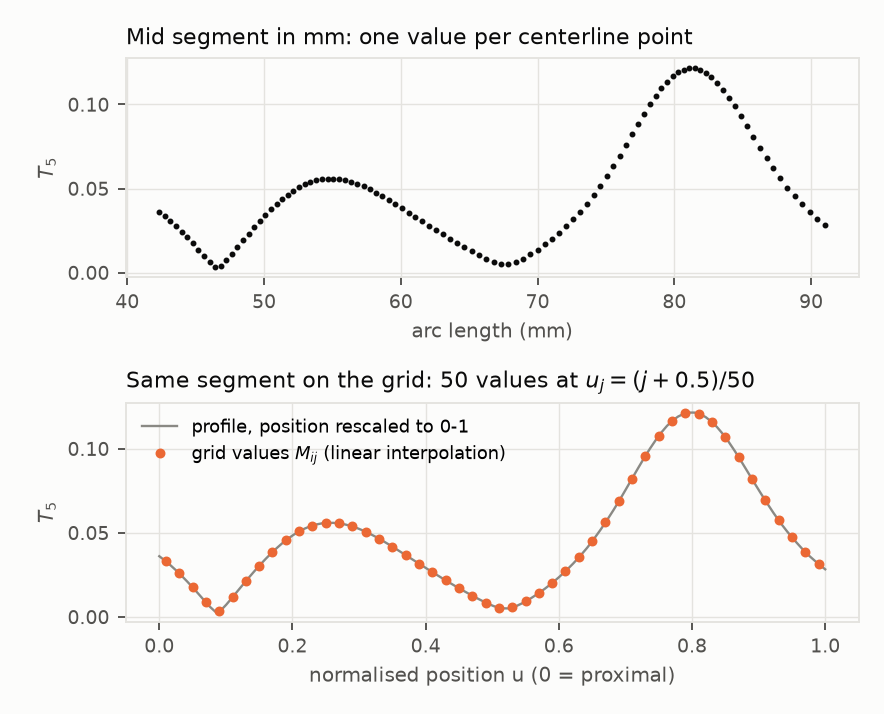
\includegraphics[width=\linewidth]{week_figure/fpca/f3_grid.png}\\[-0.1em]
{\footnotesize One made-up segment in mm (top) and read at the 50 places (bottom).}
}

\fpcarow{%
\textbf{Turning curves and deviations.} Each person is now one curve of 50 values (top, grey). The average curve (black) says how much everybody turns at
each place, for example that everybody turns more near the start. It is the same for everyone, so it
cannot tell people apart. At each place the average there is subtracted from everyone. What is left,
the deviation (bottom), is how much and where each person turns more or less than the average person. Where the bundle is wide, people
differ a lot. A bend covers several neighbouring places, so these places go up and down together
across people; FPCA looks for such groups of places, and each group becomes a shape.
}{%
\fpcafig{f4_profiles_deviations.png}{Turning curves of made-up people with their average (top), and
the same curves minus the average (bottom).}
}

\fpcarow{%
\textbf{Shapes, one at a time.} The first shape is the pattern along which people differ most (top
left). Each person has some amount of it, their score, and when that amount is taken away, less of the
differences is left (top right). The next shape is found in what is left, and so on, so each shape
describes something the earlier ones do not. Here the first shape is almost flat and positive, and
the next shapes say \emph{where} a person turns: more at the start than at the end, or more in the
middle than at the ends.

\medskip
\textbf{Number of shapes.} After the real shapes, new shapes only describe noise. Three checks decide
where to stop: whether a shape explains more than it would by chance, whether it comes back when the
people are redrawn, and how many shapes best predict a hidden part of a curve. The smallest of the
three is used, and it is fixed before plaque is looked at, so the choice cannot be tuned to find an
effect.
}{%
\fpcafig{f6_steps.png}{Left: what is not yet explained, with the next shape. Right: what is left.}
}

\textbf{A flat first shape is the mean turning.} The first shape is the main way in which people's
curves differ. When it is flat, that difference is the same all along the segment: a person who turns
more than average at the start also tends to turn more than average in the middle and at the end, by
about the same amount. Drawn as the average plus and minus the shape, it gives two curves parallel to
the average, one above and one below. The largest difference between people is then not \emph{where}
they bend but \emph{how much} they bend overall, which is exactly what the mean turning measures. Here
the first shape is only nearly flat, yet the score on it and the mean turning correlate 0.998.

\textbf{We see the same in the Herlev--{\O}sterbro data.} In the Medis centerlines the first shape has
the same sign along the whole segment and is close to a straight line, and explains the largest
share of the differences, so the mean turning captures most of what separates them.
The Medis trees come from participants with plaque at baseline, so this must be confirmed in the
plaque-free cohort.
\par\medskip

\fpcarow{%
\textbf{From scores to the risk model.} The shapes are the same for everyone; a person's score says
how much of a shape they have. It is found by comparing the person's curve with the shape at every
position: the more they match, the higher the score. A person who follows the shape gets a positive
score, one who does the opposite a negative score, and the average person 0. The average plus each
shape times its score rebuilds the curve (top), so a few scores replace the 50 numbers and go into the
risk model of the segment, next to SCORE2:
\[
  \mathrm{cloglog}(p_i) = a + g\,\mathrm{SCORE2}_i + \sum_{k} b_k\, z_{ik},
\]
where $p_i$ is the risk that person $i$ develops plaque in the segment and $e^{b_k}$ the hazard ratio
per SD of shape $k$. The weights read back as one weight per place (bottom). They are not estimated
yet, so which parts of each shape raise or lower the risk is unknown.
}{%
\centering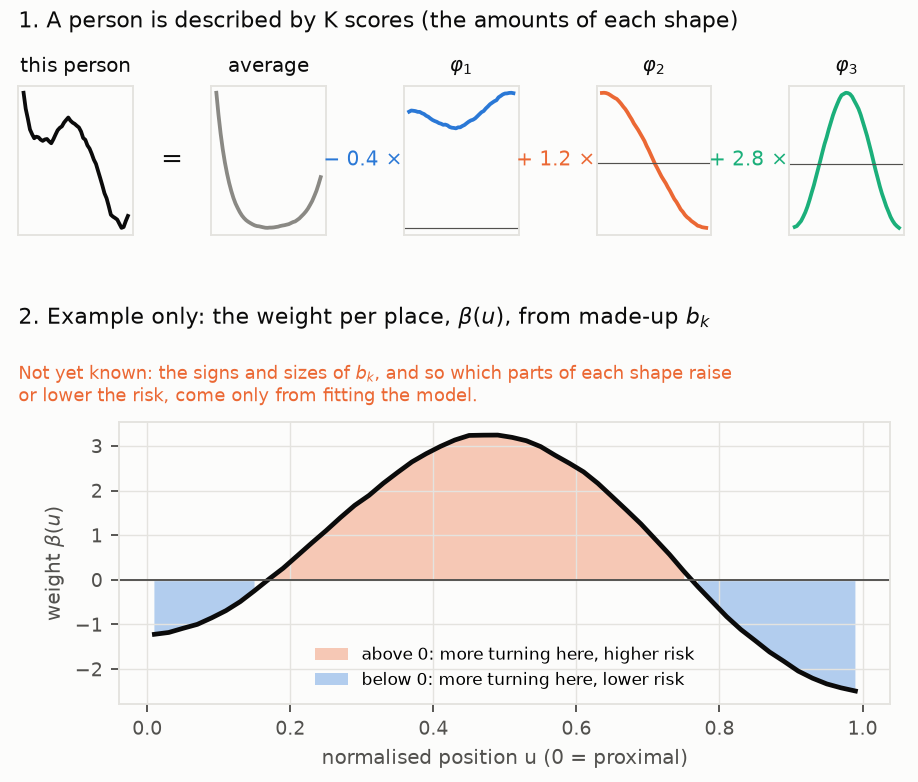
\includegraphics[width=0.88\linewidth]{week_figure/fpca_steps/fake/p3_story.png}\\[-0.1em]
{\footnotesize Top: one made-up person as the average plus scores times shapes. Bottom: made-up
weights; the real signs are not yet known.}
}

\textbf{The end goal.} The aim is to see whether some patterns of turning carry more risk than others,
that is, whether the weights of some shapes have more predictive value than others. A person who turns
a lot at the start of the segment and hardly at all after it may carry more risk than a person who
turns a little the whole way along, even with the same mean turning, and the mean turning cannot tell
these two apart. The main model keeps the mean turning: it was chosen beforehand, as earlier studies
point to it and it explains most of the differences between people, and it is not changed after this
analysis, to avoid choosing the model by its p-values.


% Week 10: the pooled segment cloglog GLMM and its person risk. Input from week10.tex.
\subsection*{From nine segment risks to one person risk}
The who question is about the person: did the participant develop plaque anywhere in the nine trunk
segments (proximal, mid and distal LAD, LCx and RCA)? The segments of one person are not independent,
since risk factors nobody measured act on all of them. The main model is a segment-level cloglog GLMM
with a person random intercept, whose segment risks are pooled into one person risk. A person-level
model of ``any plaque'' is robust but carries little information on effects that act on a few
segments only, such as the LM angle; it is kept as the benchmark. Multiplying the risks of separate
segment models ignores the shared person effect and overestimates the person risk; a logit GLMM gives
no simple person risk; GEE gives none at all; and a count model of segments with plaque cannot use
segment geometry. The pooling rule is fixed before any outcome is seen: the rule alone can move a
person-level AUC by several hundredths, so choosing it afterwards would be a hidden multiple test.

\subsection*{Why the complementary log-log link}
\textbf{One coefficient means the same in every segment.} The pLAD develops plaque far more often than
the dLCx. Under the cloglog link, $e^{\beta}$ is a hazard ratio and multiplies the rate of plaque onset
by the same factor whatever the segment's baseline risk. An odds ratio does not stay fixed: a hazard
ratio of 1.5 is an odds ratio of 1.50 at a baseline risk of 1\,\%, 1.54 at 10\,\% and 1.83 at 50\,\%
(Figure~\ref{fig:hrvsor}).

\textbf{Hazards add, so the nine segments collapse into one number.} Given the person effect, the
probability of no plaque in any segment is $\exp(-\sum_j \Lambda_j)$. The person risk depends on the
tree only through the summed hazard $S_i = \sum_j \Lambda_{ij}$, so the person-level model is itself a
cloglog model, and an unevaluable segment simply drops out of the sum.

\textbf{It matches the data.} Each segment is plaque-free at baseline and seen again about ten years
later, with the onset time unknown. This is grouped survival data, for which the cloglog model is the
proportional hazards model (Prentice and Gloeckler 1978). Log segment length enters as exposure.

The segment model also gives more precise geometry coefficients for local effects, which are seen as
contrasts between segments of the same person; it does not by itself improve discrimination. The cost
is that the person risk is only as good as the segment model: segments independent given the person
effect, a normal person effect and the same hazard ratio in every segment.

\begin{figure}[h]
  \centering
  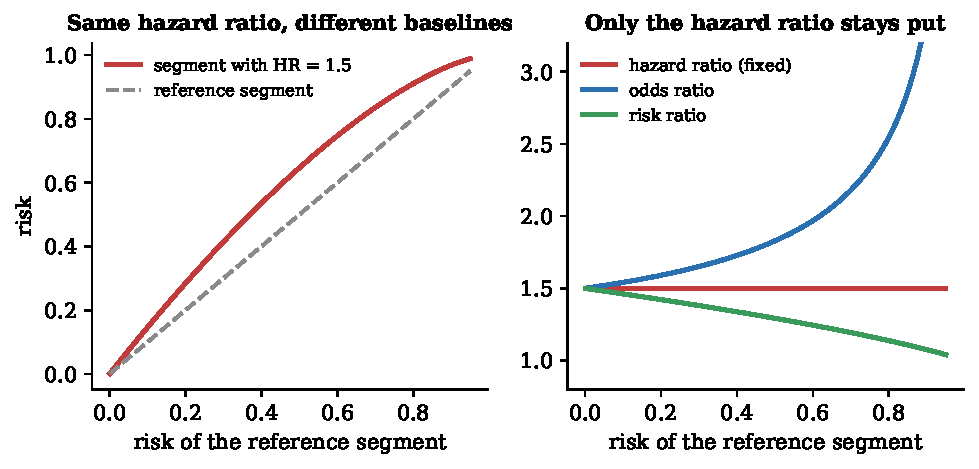
\includegraphics[width=0.85\textwidth]{week_figure/pooled/f06_hr_vs_or.pdf}
  \caption{One risk factor with a fixed hazard ratio of 1.5, made-up numbers. Left: the risk of the
           exposed segment against the risk of the reference segment. Right: the hazard ratio stays
           fixed while the odds ratio and the risk ratio drift with the baseline risk.}
  \label{fig:hrvsor}
\end{figure}

\subsection*{The model}
Each person contributes nine rows, one per trunk segment, with the score
\begin{equation}
  \begin{split}
  \eta_{ij} = {} & \alpha_j + \beta_\mathrm{S}\,\mathrm{SCORE2}_i + \beta_\mathrm{L}\log(\text{length}_{ij})
                 + \beta_\mathrm{c}\, z^\mathrm{curv}_{ij} + \beta_\mathrm{t}\, z^\mathrm{taper}_{ij} \\
               & + \beta_\mathrm{a}\, z^\mathrm{LM\,angle}_i\,[j \in \{\mathrm{pLAD}, \mathrm{pLCx}\}]
                 + \beta_\mathrm{d}\, z^{\mathrm{LM}\to\mathrm{LAD}}_i\,[j \in \mathrm{LAD}]
                 + \beta_\mathrm{x}\, z^{\mathrm{LM}\to\mathrm{LCx}}_i\,[j \in \mathrm{LCx}] .
  \end{split}
  \label{eq:eta}
\end{equation}
$\alpha_j$ is one intercept per segment. Curvature and taper are $z$-scored within segment type. The
three LM features are measured once per person and enter only on the rows downstream of the
bifurcation; $[\cdot]$ is 1 when the condition holds. The five geometry weights form the geometry block.
The segment risk is
\begin{equation}
  P(\text{segment } j \text{ of person } i \text{ develops plaque} \mid b_i)
    = 1 - \exp\!\big(-e^{\eta_{ij} + b_i}\big),
  \qquad b_i \sim N(0, \sigma^2),
  \label{eq:cloglog}
\end{equation}
where the person effect $b_i$ multiplies all nine hazards of a person by $e^{b_i}$. Only $\sigma$ is
estimated. For a new person $b$ is unknown, so the person risk averages over it:
\begin{equation}
  P_i = 1 - \int \exp\!\big(-e^{b} S_i\big)\, \phi(b; 0, \sigma^2)\, \mathrm{d}b ,
  \qquad S_i = \sum_j e^{\eta_{ij}} ,
  \label{eq:personrisk}
\end{equation}
computed by Gauss--Hermite quadrature with 40 points.

\textbf{Worked example (made-up numbers).} Toy person A has a summed hazard $S_\mathrm{A} = 0.763$, of
which the pLAD contributes 0.278. With $\sigma = 1.1$, $P_\mathrm{A} = 0.548$. Setting $b = 0$ gives
0.534, the risk of the median person, and multiplying the average segment risks gives 0.687
(Figure~\ref{fig:shortcuts}). Both shortcuts rank people correctly, so only calibration detects them.
A pLAD hazard ratio of 1.3 raises A's summed hazard by about 11\,\%, not 30\,\%, which is why segment
geometry moves the person risk only a little.

\begin{figure}[h]
  \centering
  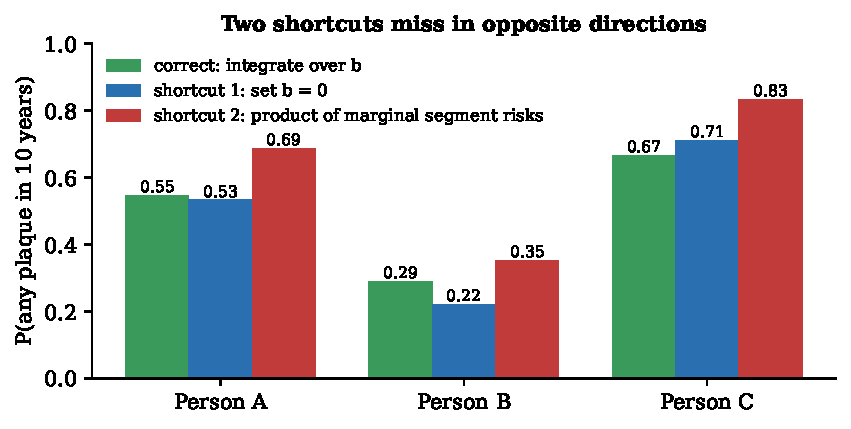
\includegraphics[width=0.75\textwidth]{week_figure/pooled/f16_shortcuts.pdf}
  \caption{Person risk of three made-up people. Green: the correct risk, averaged over the person
           effect $b$. Blue: $b$ set to 0. Red: product of the average segment risks.}
  \label{fig:shortcuts}
\end{figure}

\textbf{Fitting and testing.} The weights and $\sigma$ are fitted by maximum likelihood with $b$
integrated out (L-BFGS-B, Gauss--Hermite quadrature). Cross-validation is split by person, and $P_i$
uses the $\sigma$ from the training folds. Geometry is tested once, by a likelihood-ratio test of the
five geometry weights against the base model (segment intercepts, SCORE2, log length, $\sigma$) on 5
degrees of freedom. The gain in person-level C and the calibration are estimated with intervals, not
tested.

\textbf{Limits.} The current code (\texttt{CGPS\_data/progression\_who\_pooled.py}) runs on the Medis
trees with progression as the outcome and a 2-degree-of-freedom geometry block (mean turning $T_5$ and
the LM angle); taper and the LM diameter ratios wait for the tracer geometry on the plaque-free
cohort. Whether SCORE2 enters as the published score or as refitted factors will be decided in this
model. A gamma person effect, which gives a closed-form risk, is a sensitivity check. The full
derivation is in \texttt{cloglog\_model\_explained.pdf}.


% TotalSegmentator -> start points -> in-house tracer (Kit Mills Bransby). Not the author's
% contribution, so only outputs and how it was run on CGPS; the author's check is sec:method-medis.
% Each red [Qn] blank is answered by Qn in the list below; fill the blanks, then delete the list.
% Red notes need \usepackage{xcolor}. Remove before submission.
\providecommand{\clarify}[1]{\textcolor{red}{\textbf{Clarification needed:} #1}}
\providecommand{\ask}[1]{\textcolor{red}{[#1]}}
\section{Coronary Centerline and Lumen Extraction}
\label{sec:method-tracer}

To extract the coronary centerlines and lumen from the baseline CCTA volumes, an in-house tracer was applied to all scans of the Herlev--{\O}sterbro cohort (Section~\ref{sec:data-cohort}). The in-house tracer was developed and run by Kit Mills Bransby. The method is described here to document the full pipeline. 


\clarify{Questions for Kit: Can you give a brief description of the tracer. Should we call it in-house tracer or do you have a better name for it? Are the centerline points smoothed before they are written out (for example averaged over neighbouring points or fitted with a spline)? If so, how, and over what width in mm? The curvature profile assumes the points arrive smoothed and does not smooth them again.}


% Comparison of the in-house tracer (sec:method-tracer) with the Medis reference (sec:data-medis).
% Shortened 2026-11-01 from the 2026-10-31 version (source: reports/Centerline and lumen contour
% comparison.md). The general definitions (correspondence, OV/OT/AI, limits of agreement) were in
% technical_background/retired/07_agreement.tex, retired 2026-11-06; the body never referenced it.
% Define limits of agreement here if they are reported. Limitations (single reader, plaque-only
% reference, shared imaging errors) go in the Discussion.
% Every threshold marked [x] is a design choice without a published value; fix it before the
% comparison is run and before any outcome analysis, never tune it on the result.
% Red clarification notes; needs \usepackage{xcolor} in the preamble. Remove before submission.
\providecommand{\clarify}[1]{\textcolor{red}{\textbf{Clarification needed:} #1}}
\section{Comparison With the Medis Reference}
\label{sec:method-medis}

No ground truth exists for the Herlev--{\O}sterbro scans, so the quality of the centerlines and lumen contours from the in-house tracer (Section~\ref{sec:method-tracer}) cannot be measured directly.
Instead, they were compared to the Medis centerlines and the semi-manually annotated Medis contours of the same baseline scans (Section~\ref{sec:data-medis}), which gives an indirect estimate.
Medis: \clarify{how were they exactly produced and handled (semi corrected?} 
Medis data exist only for participants with plaque at baseline, so the comparison was made outside the plaque-free study cohort.

\subsection{Medis Centerlines as Full Arteries}
\label{sec:method-medis-arteries}
The tracer and Medis label their centerlines at different levels.
Medis labels each point of its centerlines with a segment, such as the \textbf{proximal} LAD, whereas the tracer labels only the artery.
To measure the tracing error rather than a difference in where the tracer and Medis place the segment boundaries, the proximal, mid and distal Medis segments of each artery were collapsed into one full artery.
This thesis uses only the LAD, LCx and RCA (Section~\ref{sec:method-population-arteries}), so the comparison was limited to these three arteries.

\subsection{Agreement Between the Tracer and Medis}
\label{sec:method-medis-agreement}
The centerlines and contours enter the prediction model only through the geometric features computed from them (Section~\ref{sec:method-features}).                                                                           
Therefore the agreement was measured on the features and not the points themselves.
First the tracer centerlines and contours were mapped into the coordinates of Medis, and each tracer artery was paired with the Medis artery of the same participant and label.
\clarify{in which coordinates are the Medis points stored: LPS millimeters, RAS millimeters or voxel indices? And in which coordinates does the tracer store its points?}

Centerline features were computed on the full artery without any adjustments, whereas the lumen contour features were computed only over the part of the artery covered by the Medis lumen contours.
To achieve this, the tracer centerline was cut where the first and the last Medis lumen contour lie \cite{schaap2009cat08}, which cut its lumen contours to the same stretch.



% Study cohort and outcome, written for a first-time reader (rewritten 2026-11-02; arteries and
% segments moved to 02b_segment_split.tex). Definitions only: the counts (flowchart, incident plaque per artery)
% are in results/00_cohort.tex (sec:results-cohort), what the visual analysis recorded is in
% data/02_visual_analysis.tex, and the overlap with the Medis trees in data/03_medis_reference.tex.
% Does not repeat data/01-03: cohort size, segment grading, SIS/SSS, Medis coverage.
% The choice of arteries (sec:method-population-arteries), why the analysis is per segment and the
% division into segments (sec:method-split) and its check (sec:method-split-validation) are in
% 02b_segment_split.tex; the landmark table is in appendix/B_segment_split_details.tex.
% Does not repeat clinical_background_v2 (sec:wss, sec:tree).
% Still open: follow-up time enters the model as log(years); missing baseline geometry (open
% decision 9); partly graded FU arteries.
% [..] and \clarify{} mark information that is not yet available; nothing there is to be guessed.
\providecommand{\clarify}[1]{\textcolor{red}{\textbf{Clarification needed:} #1}}
\section{Study Cohort and Outcome}
\label{sec:method-population}

The study cohort comprised the Herlev--{\O}sterbro participants without coronary plaque at baseline, defined by a segment involvement score (SIS) of zero (Section~\ref{sec:data-plaque-location}).
Participants with insufficient image quality ([criterion]) were also excluded, and the resulting cohort is described in Section~\ref{sec:results-cohort}.
The primary outcome was incident coronary plaque, defined at the segment level as a stenosis grade of minimal or worse and at the participant level as plaque in at least one of the analysed segments (Section~\ref{sec:method-population-arteries}).
In a sensitivity analysis, the outcome was restricted to plaque with mild or worse stenosis.
% Counts (65 RCAs, 5 LCxs, <5 LADs) belong in results/00_cohort.tex, not yet there.

\clarify{The outcome could still change!!!}


% Coronary segments: the choice of arteries, their division into proximal, mid and distal
% segments, and a check of the division. Short main text (user, 2026-11-02): the exact division,
% thresholds and the landmark table are in appendix/B_segment_split_details.tex (sec:app-split).
% Placed after 02_population_outcome. Humanised 2026-11-02 in the style of clinical_background_v2.
% Does not repeat: tracer labels only the artery, Medis by segment (01b, sec:method-medis-arteries);
% what the visual analysis and the Medis trees and contours are (data/02, data/03).
% Division: CGPS_data/split_trunks.py (landmark_cuts). Check: CGPS_data/thesis_final/split_check.py
% --trees tracer, section 2 (contours by location vs the visual BL grade: a contour whose majority
% segment is not graded plaque = miss); reference run --trees medis.
% Red clarification notes; needs \usepackage{xcolor} in the preamble. Remove before submission.
\providecommand{\clarify}[1]{\textcolor{red}{\textbf{Clarification needed:} #1}}
\section{Analysed Arteries and Segments}

\subsection{Choice of Arteries}
\label{sec:method-population-arteries}

The analysis covered the three main coronary arteries, the left anterior descending (LAD), the left circumflex (LCx) and the right coronary artery (RCA), both for the outcome and for the geometric features.
These arteries are present in every heart, whereas the number and size of the side branches vary between individuals and with dominance (Section~\ref{sec:dominance}).
Their larger diameter also makes the measurements less sensitive to error: with a voxel size of [..]\,mm, an error of one voxel at the lumen boundary corresponds to about [..]\% of the diameter of a main artery \cite{dodge1992diameter}, compared with [..]\% for a side branch \clarify{voxel size; side-branch diameter and its citation}.
The left main (LM) was also left out.
None of the studies in the literature review related LM geometry to plaque in the LM itself; the angle of the LM bifurcation was instead related to disease further down, in the LAD and LCx (Chapter~\ref{ch:literature}).
A participant who developed plaque only in the LM or in a side branch was therefore counted as without the outcome.
This applied to a small proportion of participants (Section~\ref{sec:results-cohort}), and the implications of this misclassification are addressed in Section~[..] \clarify{discussion section on this misclassification, not yet written}.                                                                           

\subsection{Division into Segments}
\label{sec:method-split}

Geometry is theorised to influence plaque formation through low wall shear stress, which is a local force. 
A feature averaged over a whole artery would risk blurring these local differences, so the features were computed at the same fine resolution as the outcome.
Each of the three arteries was therefore divided into a proximal, a mid and a distal segment, giving nine segments per participant (Figure~\ref{fig:method-segments}).

The visual analysis does not record where one segment ends and the next begins, so a landmark division method was developed and used in this thesis to place the boundaries.
Where no such branch was available, the boundary was placed at a fixed fraction of the distance along the artery.
The full division is given in Appendix~\ref{sec:app-split}.

% Figure from segment_selection_schematic.py (made-up tree, no patient data).
\begin{figure}[htbp]
  \centering
  \includegraphics[width=\textwidth]{methodology/segment_selection_schematic.pdf}
  \caption{From the graded coronary segments to the nine segments. (A) The segments graded in the visual analysis. (B) The LAD, LCx and RCA retained; the left main and the side branches are shown in light grey. (C) Each retained artery divided into a proximal, a mid and a distal segment at the landmarks of Table~\ref{tab:method-segments}. D1 and D2, diagonal branches; IM, intermediate branch; OM1 and OM2, obtuse marginal branches; PDA, posterior descending artery; PLA, posterolateral branch. Schematic, not to scale.}
  \label{fig:method-segments}
\end{figure}

\subsection{Validation of the Division}
\label{sec:method-split-validation}

To give an indication of the reliability of the division, the Medis lumen contours were projected onto the nearest points of the divided tracer artery, and the segment holding the largest part of each contour was looked up in the visual analysis.
If that segment was not graded with plaque at baseline, a miss was recorded.
Only the position of the contour was used, not the segment name Medis gave it, so the check does not depend on how Medis divided the artery.
The miss rate is reported in Section~\ref{sec:results-cohort}.
A slightly displaced boundary moves only a few points at either end of a segment, so features computed per segment were preferred, despite this uncertainty, to features averaged over the whole artery.


\end{document}
